\begin{center}
    \section{Семинар III}
\end{center}
\subsection{Эволюция квантовых систем. Уравнение Шрёдингера}
\hspace{1em} Перед тем, как начать обсуждать динамику квантовых систем, важно обговорить одно исключение: время в квантовой механике не рассматривается как оператор. Не существует ни собственных состояний времени ни квантового времени. Время – просто непрерывная переменная.

Теперь перейдём к эволюции квантовых объектов. Поставим задачу: при заданном начальном состоянии $\ket{\psi(0)}$ системы нужно определить её состояние $\ket{\psi(t)}$ в произвольный момент времени. Решение этой задачи не получится вывести из аппарата, который у нас есть на данном этапе, поэтому постулируем, что эволюция системы будет описываться следующим уравнением:
\[
\ket{\psi_E(t)} = \ket{\psi(0)} e^{-\frac{i}{\hbar} E t}.
\]
Это уравнение имеет место, когда система находится в состоянии с определенной энергией.

В классической механике для описания динамики системы достаточно было знать \textit{гамильтониан} системы. В квантовой механике всё работает примерно так же, только гамильтониан надевает шляпку и становится оператором $\hat{H}$. Как и у любого оператора, у гамильтониана есть свои собственные состояния и собственные значения. Логично предположить, что эти значения и состояния будут соответствовать определенным значениям энергии:
\[
\hat{H} = \sum_j E_j \ket{E_j} \bra{E_j}.
\]
Тогда, любое состояние может быть разложено в этом базисе:
\[
\ket{\psi(0)} = \sum_j \psi_j \ket{E_j}.
\]
Собственные энергетические состояния называют \textit{стационарными}. Исходя из введённого выше постулата, эволюция системы будет описываться уравнением:
\[
\ket{\psi(t)} = \sum_j \psi_j \ket{E_j} e^{-\frac{i}{\hbar} E_j t}.
\]
С помощью этого уравнения можно вычислять эволюции состояния, однако на практике мы чаще будем пользоваться двумя другими уравнениями, о которых сейчас поговорим.

Мы уже привыкли пользоваться операторами для изменения состояния системы. Давайте и здесь введём унитарный оператор для описания эволюции системы. Унитарность здесь важна, в том числе для того, чтобы все преобразования были обратимы относительно эрмитового сопряжения. Такой оператор мы назовём \textit{оператором эволюции} $\hat{U}$. Он будет удовлетворять уравнению:
\[
\ket{\psi_E(t)} = \hat{U} \ket{\psi(0)}
\]
В явном виде матричный элемент оператора эволюции выглядит как:
\[
U_{jk} = \bra{E_j} \hat{U} \ket{E_k} = e^{-\frac{i}{\hbar}E_k t} \bra{E_j} \ket{E_k} = e^{-\frac{i}{\hbar} E_k t}\delta_{jk}.
\]
Или, если записать это в бракет нотации:
\[
\hat{U} = \sum_{k} e^{-\frac{i}{\hbar} E_k t} \ket{E_k} \bra{E_k}.
\]
Чтобы получить итоговый вид оператора эволюции, перепишем его через оператор гамильтониана: 
\[
\hat{U} = e^{-\frac{i}{\hbar} \hat{H} t}
\]
Чтобы получить последнее, самое важное уравнение, продифференцируем состояние, полученное применением оператора эволюции на начальное состояние:
\[
\frac{d}{dt} e^{-\frac{i}{\hbar} \hat{H} t} \ket{\psi(0)} = -\frac{i}{\hbar} \hat{H} e^{-\frac{i}{\hbar} \hat{H} t} \ket{\psi(0)} = -\frac{i}{\hbar} \hat{H} \ket{\psi(t)}.
\]
Если оставить справа только оператор гамильтониана, то мы получим \textit{уравнение Шрёдингера}:
\[
i \hbar \frac{d}{dt} \ket{\psi(t)} = \hat{H} \ket{\psi(t)}.
\]
В общем случае гамильтониан также может зависеть от времени, но этот случай мы рассмотрим позднее. Пока наша задача в том, чтобы найти множество собственных значений и состояний гамильтониана. Т.е. нужно найти состояния $\ket{\psi}$, такие что:
\[
\hat{H} \ket{\psi} = E \ket{\psi}.
\]
Это уравнение называется \textit{стационарным уравнением Шрёдингера}. Так, для гамильтониана частицы в поле $\hat{H} = V(\hat{x}) + \hat{p}^2 / 2M$, где первый член -- это потенциальная энергия, а второй -- кинетическая, стационарное уравнение Шрёдингера, будет выглядеть следующим образом:
\[
\left[V(x) - \frac{\hbar^2}{2M} \frac{d^2}{dx^2}\right] \psi(x) = E \psi(x).
\]
Здесь мы перешли от вектора состоянии к волновой функции, домножив слева на бра состояние $\bra{x}$.

Можно сказать, что теорминимум был нами освоен и можно приступать к решению первых содержательных задач. В целом, решение большинства задач в курсе по квантовой механике сводится к решению либо стационарного либо зависящего от времени уравнения Шрёдингера. Поэтому запоминаем его, записываем на обложках тетрадей, делаем татуировки и т.п. Чтобы помочь вам запомнить, решим несколько задач на потенциальные ямы. Этот тип задач основан на том, что мы решаем стационарное уравнение Шрёдингера, но с разным потенциалом. В общем, хватит слов, переходим к задаче.
\excersize{Упражнение №12}{darklavender}
\begin{center}
    \textit{Частица массы m совершает финитное движение в одномерной ``прямоугольной'' потенциальной яме конечной глубины:}
    \[
    U(x) = 
    \begin{cases}
    -U_0,& |x| < a,\\
    0, & |x| > a.
    \end{cases}
    \]
    \textit{Найдите уровни энергии $E_n$ и волновые функции $\psi_n(x)$ стационарных состояний}
\end{center}

Для начала разберёмся с условием. \textit{Связанные состояния} – состояния, для которых волновая функция при $x \rightarrow \pm \infty$ равна $0$. Получается, состояние как бы локализовано в определенном объёме пространства. Из-за наложенных ограничений связанные состояния имеют \textit{дискретный спектр} собственных значений энергии, которые называют энергетическими уровнями.

На рисунке \ref{fig 3.1} можно посмотреть, как выглядит яма из задачи. Думаю, уже сейчас понятно, насколько это модельная задача. Но для понимания поведения частиц, хорошо описываемых уравнением Шрёдингера, она незаменима.
\begin{figure}[!ht]
\centering
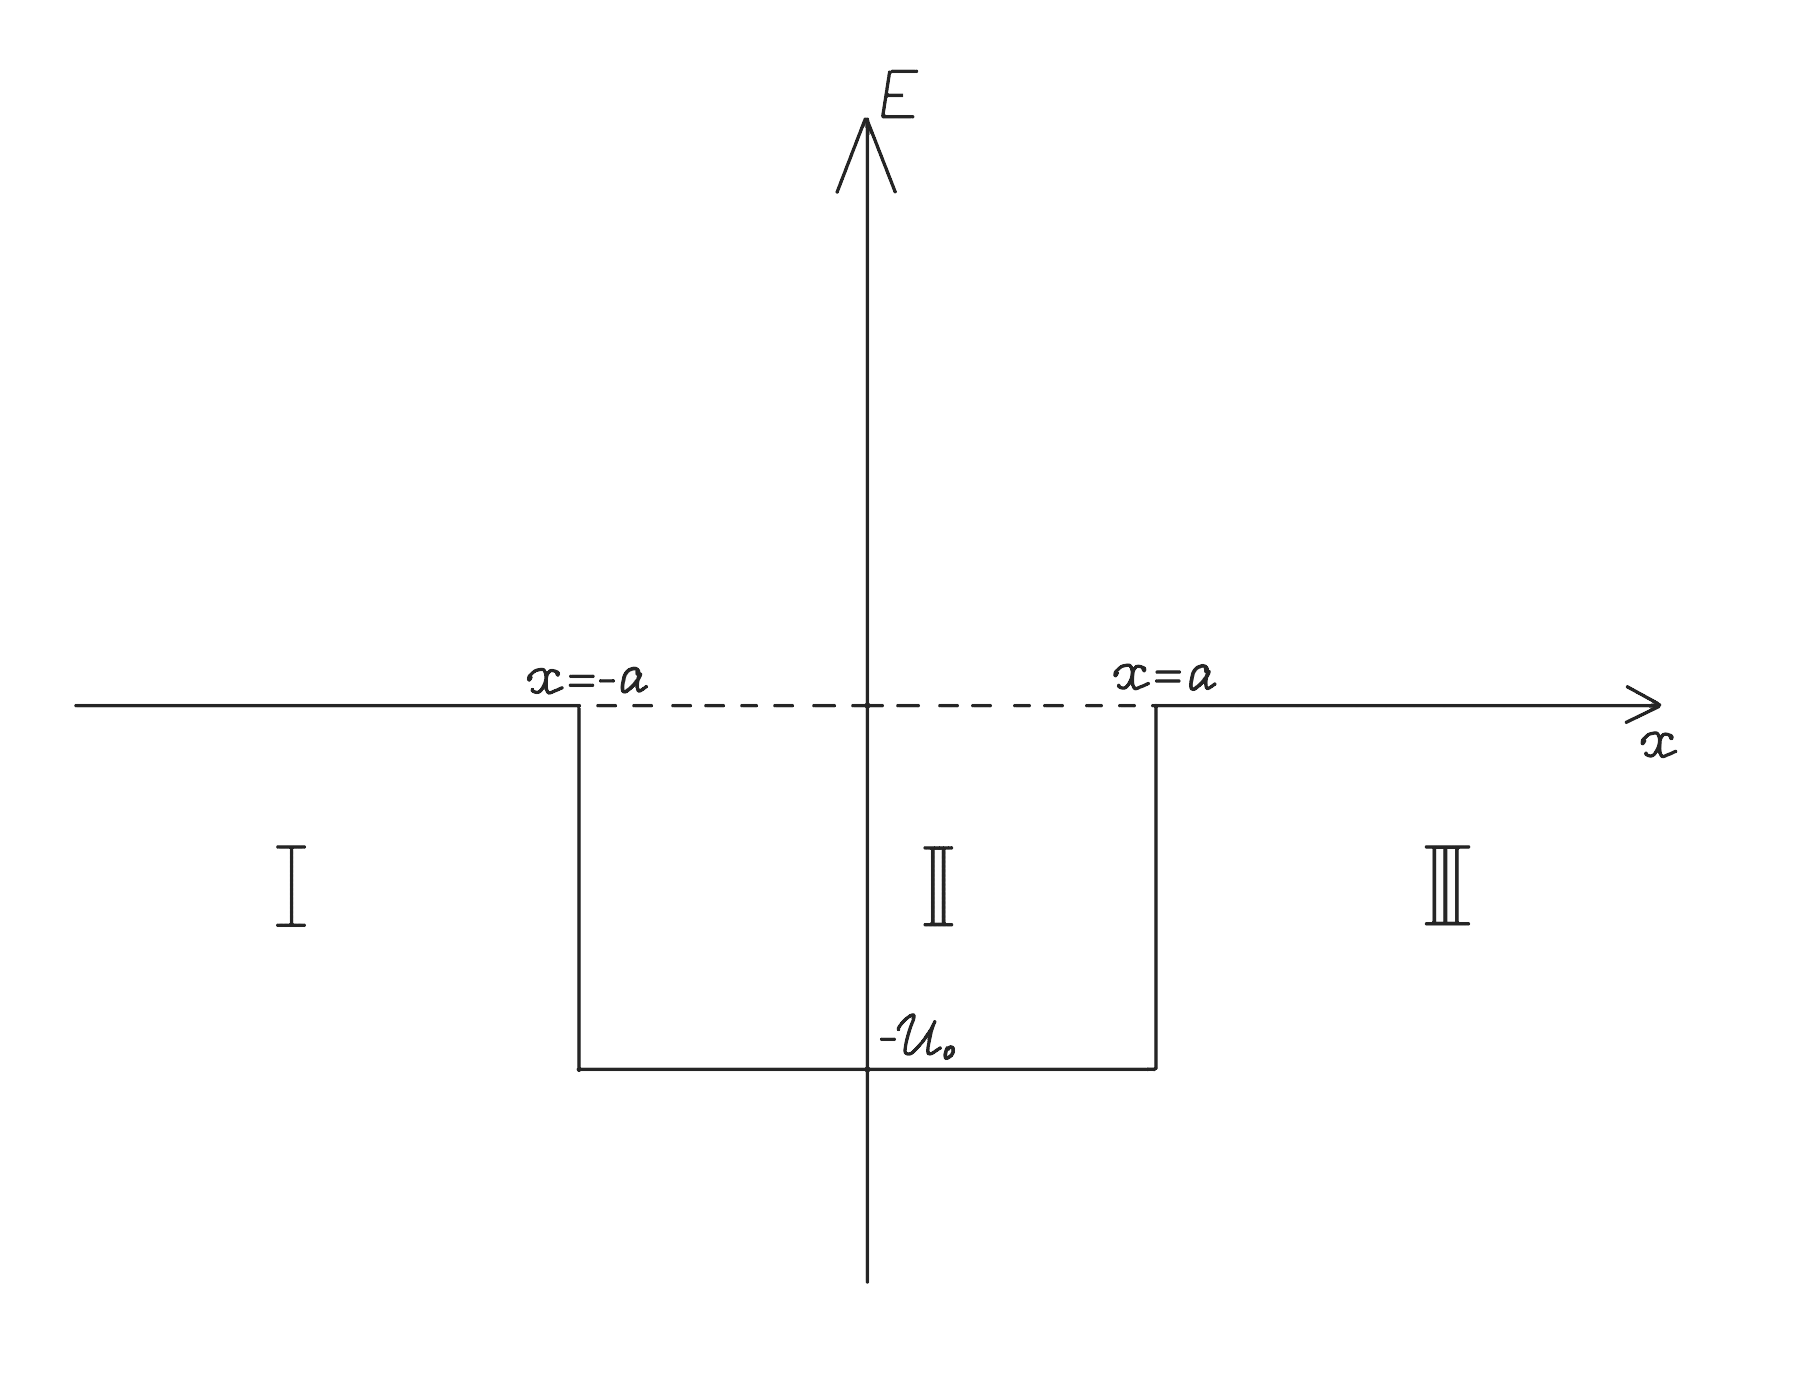
\includegraphics[scale=0.27]{class_3/images/hole.png}
\caption{Прямоугольная и симметричная потенциальная яма}
\label{fig 3.1}
\end{figure}

Выпишем одномерное стационарное уравнение Шрёдингера:
\[
U(x) \psi(x) - \frac{\hbar^2}{2m} \psi''(x) = E \psi(x).
\]
Перепишем его так, чтобы в правой части остался только 0:
\[
\psi''(x) + \frac{2m}{\hbar^2} (E - U) \psi(x) = 0
\]
Теперь давайте по отдельности рассмотрим каждую из трёх областей. В первой области (т.е. в области $x < -a$) потенциальная энергия нулевая. Так как мы рассматриваем случай финитного движения, частица не может оказаться над потенциальной энергией в непрерывном спектре. Значит, энергия частицы меньше нуля. В классическом случае мы бы с уверенностью сказали, что в этой области частица присутствовать не может. Но в квантовой механике не всё так гладко. Давайте решим стационарное уравнение Шрёдингера для этого случая:
\[
\psi_I'' - \kappa^2 \psi_I = 0, \quad \kappa^2 = \frac{2m}{\hbar^2} |E|
\]
$\kappa$ -- величина действительная, так как связана с энергией. Значит, корень нужно брать из положительного числа. Поэтому энергию мы берём по модулю. Это гармоническое уравнение, только с минусом. Решение такого уравнения известно и выражается в виде суммы двух экспонент с разными знаками:
\[
\psi_I (x) = A e^{\kappa x} + \widetilde{A} e^{-\kappa x}
\]
Оказывается, что второй член из этого уравнения выпадает. Это связанно с условием нормировки -- волновая функция при $x \rightarrow -\infty$ не должна уходить в бесконечность. Тогда мы видим, что волновая функция для первой области имеет следующий вид:
\[
\psi_I (x) = A e^{\kappa x},
\]
Получается, функция затухает экспоненциально и на минус бесконечности уходит в ноль.

Думаю, понятно, что для третьей области решение будет аналогично. Для тренировки можете проделать все выкладки самостоятельно, я же выпишу только ответ:
\[
\psi_{III}(x) = D e^{-\kappa x}
\]
Теперь выпишем уравнение для второй области:
\[
\psi_{II}'' + k^2 \psi_{II} = 0, \quad k^2 = \frac{2m}{\hbar^2}(U_0 - |E|)
\]
Соответственно, решение для него:
\[
\psi_{II}(x) = B \cos kx + C\sin kx
\]

Для дальнейших рассуждений нам понадобится важный теоретический факт о том, что, если операторы коммутируют, то у них существует общий базис собственных функций. Далее, исходя из симметрии задачи ($U(x) = U(-x)$), понимаем, что оператор инверсии может коммутировать с гамильтонианом. Проверим:
\[
[\hat{H}, \hat{I}] = [U(x) + \frac{\hat{p}^2}{2m}, \hat{I}] = [U(x), \hat{I}] + \frac{1}{2m} [\hat{p}^2, \hat{I}] = 0
\]
Значит, можно искать собственные функции гамильтониана как собственные функции оператора инверсии. Но мы знаем, что для оператора инверсии собственные функции обладают определенной чётностью. Тогда найдём чётные и нечётные волновые функции нашей задачи:
\[
\psi_+ =
\begin{cases}
    Ae^{\kappa x}& x < -a,\\
    B \cos kx & -a < x < a,\\
    Ae^{-\kappa x}& x > a
\end{cases}\quad
\psi_- =
\begin{cases}
    -De^{\kappa x}& x < -a,\\
    C \sin kx & -a < x < a,\\
    De^{-\kappa x}& x > a
\end{cases}
\]
Думаю, понятно, откуда взялись функции с синусом и косинусом. Чуть меньше ясности может быть с оставшимися функциями. Они связаны с самим определением четной функции: $Ae^{\kappa x}$ получаем из решения уравнения Шрёдингера, нужно составить такую функцию, которая при изменении знака икс не будет менять знак выражения. Получается $Ae^{-\kappa x}$. То же самое для второго: $De^{-\kappa x}$ есть, $-De^{\kappa x}$  дополняем для нечетности функции.

Рассмотрим условия на волновую функцию. Пока что она не определена на границах. То есть нужно ввести условия ``сшивки''. Их берем из физического смысла волновой функции, а именно:
\[
\psi(x) - \text{непрерывна},\; \frac{\psi'(x)}{\psi(x)} - \text{непрерывна}
\]
Из этих условий ``сошьём'' границы для чётных и нечётных функций отдельно. Так как потенциал симметричен, достаточно рассмотреть только одну границу.
\begin{gather*}
    \frac{\psi'_+(x)}{\psi_+(x)}\bigg|_{x=a-0} = \frac{\psi'_+(x)}{\psi_+(x)}\bigg|_{x=a+0} = \frac{-Bk\sin ka}{B\cos ka} = \frac{-\kappa A e^{-\kappa a}}{Ae^{-\kappa a}} \implies \\
    \implies k\tg ka = \kappa
\end{gather*}
Для нечётных:
\begin{gather*}
    \frac{\psi'_-(x)}{\psi_-(x)} \bigg|_{x = a - 0} = \frac{\psi'_-(x)}{\psi_-(x)} \bigg|_{x = a + 0} = \frac{C k \cos ka}{C \sin ka} = \frac{-\kappa D e^{-\kappa a}}{D e^{-\kappa a}} \implies \\
    \implies k \ctg ka = -\kappa
\end{gather*}
Ещё немного повертим выражение и придём к итоговому, красивому виду:
\begin{gather*}
    \text{Пусть } (\kappa a)^2 = (k_0a)^2 - (ka)^2, \; \text{где} \;k_0^2 = k^2 + \kappa^2 \\
    \kappa a = \sqrt{(k_0a)^2 - (ka)^2} \implies ka\tg ka = \sqrt{(k_0a)^2 - (ka)^2} \implies \\
    \implies \tg ka = \sqrt{\frac{(k_0a)^2}{(ka)^2} - 1}
\end{gather*}
Пользуясь тригонометрией, выразим квадрат тангенса через косинус:
\begin{gather*}
    \tg^2 ka = \frac{1}{\cos^2 ka} - 1 \implies
    \frac{1}{\cos^2 ka} - 1 = \frac{(k_0 a)^2}{(ka)^2} - 1 \implies \\
    \implies \cos^2 ka = \frac{(ka)^2}{(k_0 a)^2} \implies |\cos ka| = \frac{ka}{k_0a}, \; \tg ka>0
\end{gather*}
Проделав аналогичные вычисления для нечётных функций, в итоге получаем компактное выражение:
\[
\begin{cases}
   |\cos ka| = \frac{ka}{k_0a},& \tg ka>0 \\
   |\sin ka| = \frac{ka}{k_0a},& \tg ka<0 \\
\end{cases}
\]
У нас получаются трансцендентные уравнения. Это значит, что просто выразить какую-либо величину из этого уравнения сложно, или даже нереально. Мы можем только проанализировать его. Например:
\begin{figure}[!ht]
  \centering
  \subfloat[График для чётных функций. Выделенные области удовлетворяют условию $\tg ka > 0$]{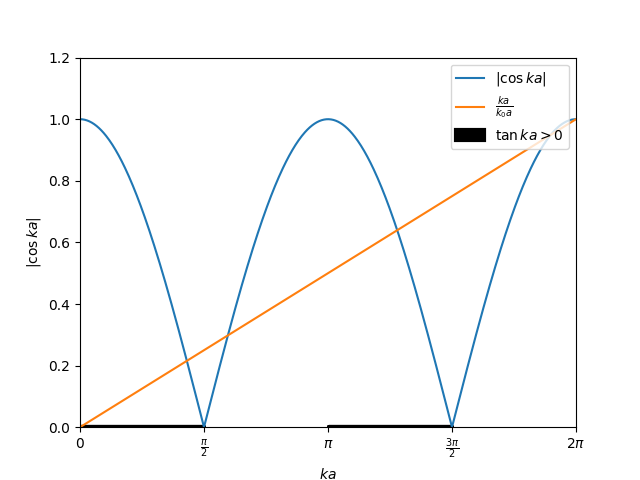
\includegraphics[scale=0.5]{class_3/images/even.png}}
  \hfill
  \subfloat[График для нечётных функций. Выделенные области удовлетворяют условию $\tg ka < 0$]{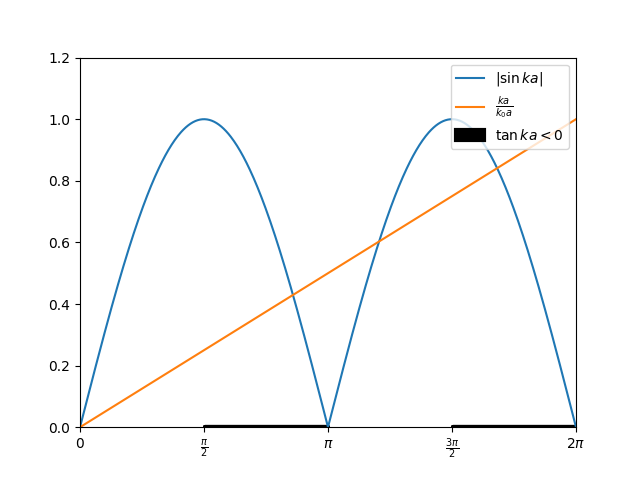
\includegraphics[scale=0.5]{class_3/images/odd.png}}
  \caption{}
\end{figure}

Что мы можем вынести из этих графиков? Для чётных функций видно, что решение существует при любом положительном $k_0a$. Так как этот параметр отвечает параметрам задачи, получается, что при любой глубине ямы у нас существует хотя бы одно чётное решение. В то же время, из графика нечётных функций достаём следующее условие существования решений: $k_0a>\frac{\pi}{2}$. Можно легко проверить, что чётные и нечётные решения чередуется. Формулы для количества решений:
\[
\left[\frac{k_0a}{\pi}\right] + 1 = N_+, \quad \left[\frac{k_0a}{\pi/2}\right] = N_-
\]
Теперь найдём коэффициенты A и B из неиспользованного условия непрерывности:
\begin{gather*}
    \psi_+(a-0) = \psi_+(a+0) \implies A = Be^{\kappa a}\cos ka \\
    \braket{\psi_+} = 1 \implies 2 * (\int\limits_0^a |B|^2\cos^2 kx dx + \int\limits_a^\infty |A|^2e^{-2\kappa x} dx) = 1 \implies \\
    \implies 2 *|B|^2 (\int\limits_0^a \cos^2 kx dx + \int\limits_a^{+\infty }\cos^2 kae^{-2\kappa(x-a)} dx) = 1 \implies \\
    \implies |B|^2 = (a + \frac{\sin 2ka}{2k} + \frac{\cos^2 ka}{\kappa})^{-1} 
\end{gather*}
Проделав ту же самую процедуру с D и C, получим:
\[
D = Ce^{\kappa a}\sin ka, \quad |C|^2 = (a - \frac{\sin 2ka}{2k} + \frac{\sin^2 ka}{\kappa})^{-1}
\]
Выпишем, какие состояния получили в итоге:
\begin{align*}
\psi_+ &=
\begin{cases}
    \sqrt{(a + \frac{\sin 2ka}{2k} + \frac{\cos^2 ka}{\kappa})^{-1}}e^{\kappa (x + a)}\cos{ka}, & x < -a,\\
    \sqrt{(a + \frac{\sin 2ka}{2k} + \frac{\cos^2 ka}{\kappa})^{-1}} \cos kx, & -a \leq x \leq a,\\
    \sqrt{(a + \frac{\sin 2ka}{2k} + \frac{\cos^2 ka}{\kappa})^{-1}}e^{\kappa (a - x)}\cos{ka},& x > a
\end{cases}\\
\psi_- &=
\begin{cases}
    -\sqrt{(a - \frac{\sin 2ka}{2k} + \frac{\sin^2 ka}{\kappa})^{-1}}e^{\kappa (x+a)}\sin ka, & x < -a,\\
    \sqrt{(a - \frac{\sin 2ka}{2k} + \frac{\sin^2 ka}{\kappa})^{-1}} \sin kx, & -a \leq x \leq a,\\
    \sqrt{(a - \frac{\sin 2ka}{2k} + \frac{\sin^2 ka}{\kappa})^{-1}}e^{\kappa (a-x)}\sin ka, & x > a
\end{cases}
\end{align*}
Всё, основную часть мы проанализировали, волновые функции и уровни энергии получили.
\csquare{darklavender}

На следующем семинаре продолжим разбирать задачи, связанные с одномерным потенциалом и уравнением Шрёдингера.
